\documentclass[12pt, letterpaper]{article}
\usepackage[utf8]{inputenc}
\usepackage[T1]{fontenc}
\usepackage{booktabs} % for borders and merged ranges
\usepackage{soul}% for underlines
\usepackage{xcolor,colortbl} % for cell colors
\usepackage{caption}
\usepackage{amsmath}
\usepackage{flafter}
\usepackage{graphicx}
\usepackage{float} % For the [H] specifier
\graphicspath{ {./images} }
\captionsetup[table]{skip=10pt}
\title{AOD - sprawozdanie nr 1}
\author{Wiktor Bachta}
\date{Październik 2024}

\begin{document}

\maketitle

\section{DFS o BFS}

\subsection{Algorytm}

Zastosowałem standardowe algorytmy DFS i BFS. Nie skorzystałem
z wersji rekurencyjnej DFS. Zastosowałem algorytm ze stosem dla DFS
i algorytm z kolejką dla BFS. W alogorytmie przy wierzchołku przechowuję
także jego rodzica (predecesor), aby można było odtworzyć drzewo
przeszukiwania. Algorytmy mają złożoność liniową - $O(V + E)$.

\subsection{Grafy}

\begin{figure}[H]
    \centering
    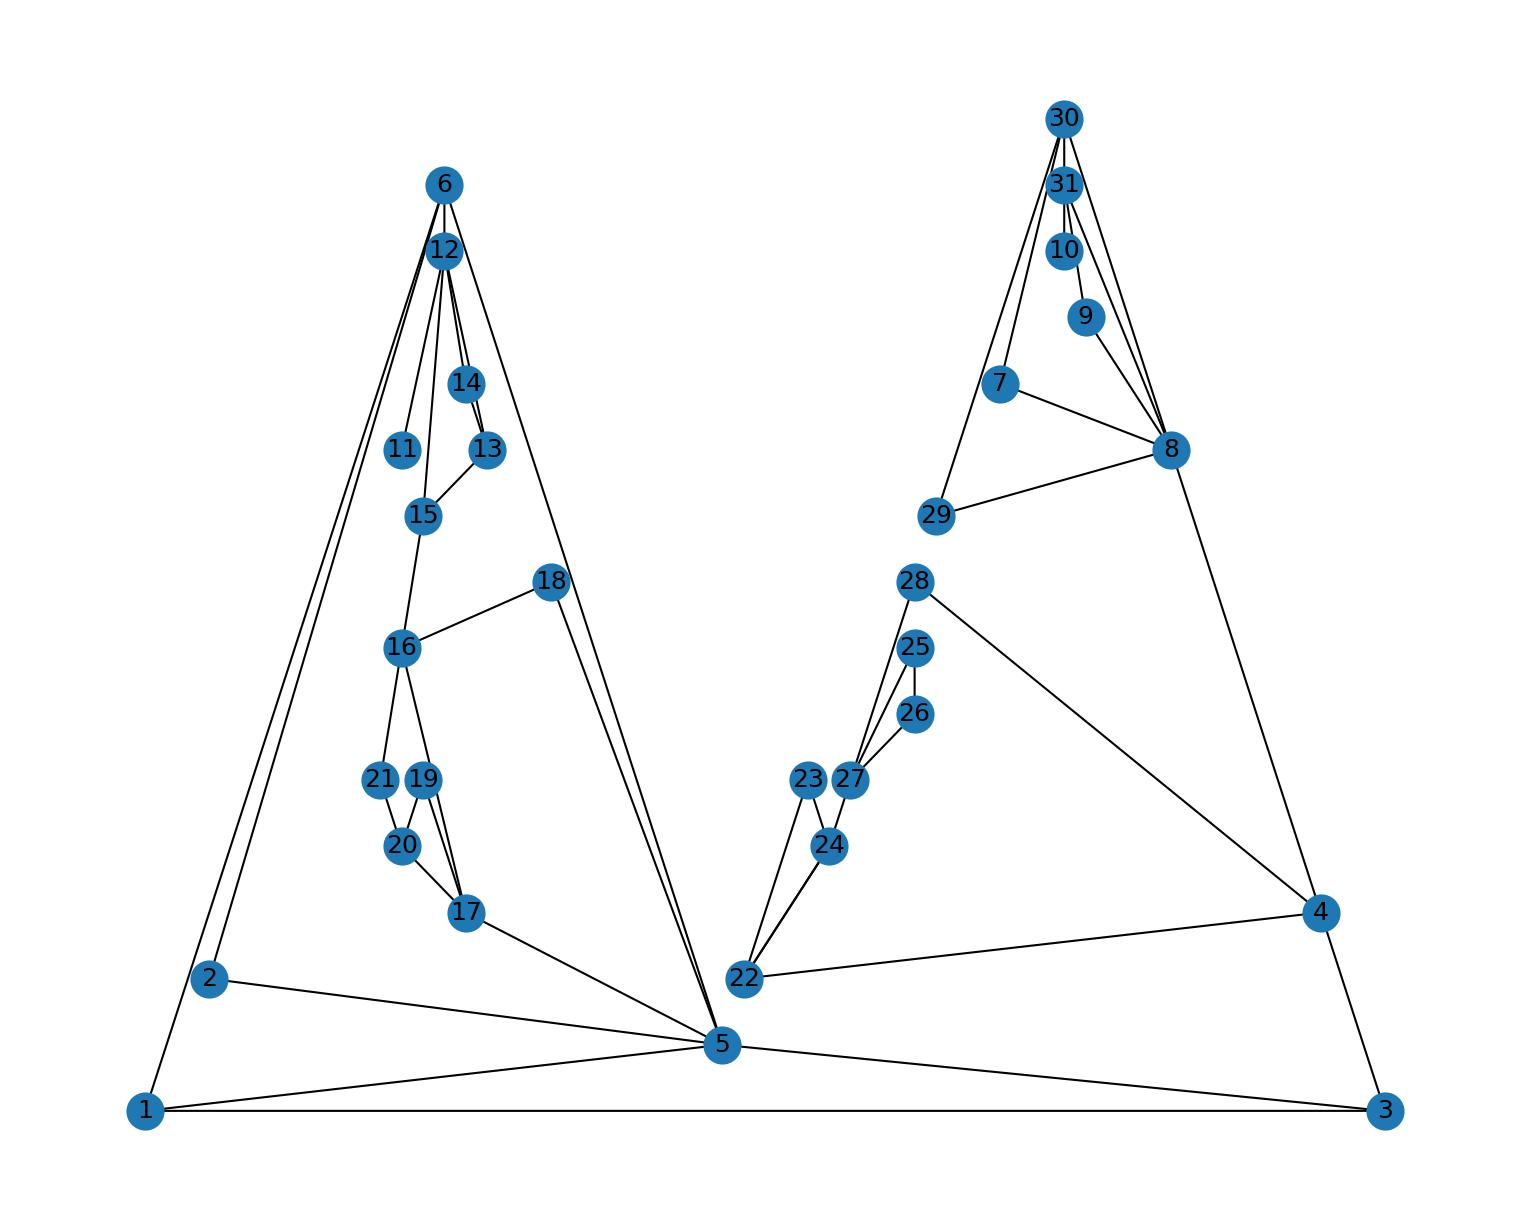
\includegraphics[width=\textwidth]{g4u.jpg}
    \caption{Graf nieskierowany}
\end{figure}

\begin{figure}[H]
    \centering
    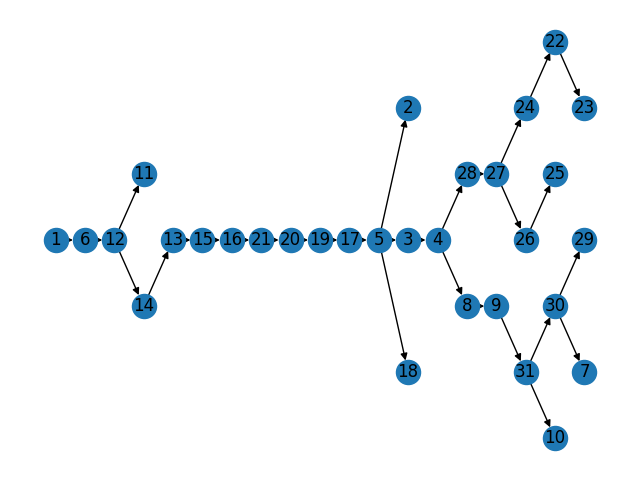
\includegraphics[width=\textwidth]{g4u-dfs.png}
    \caption{Drzewo DFS}
\end{figure}

\begin{figure}[H]
    \centering
    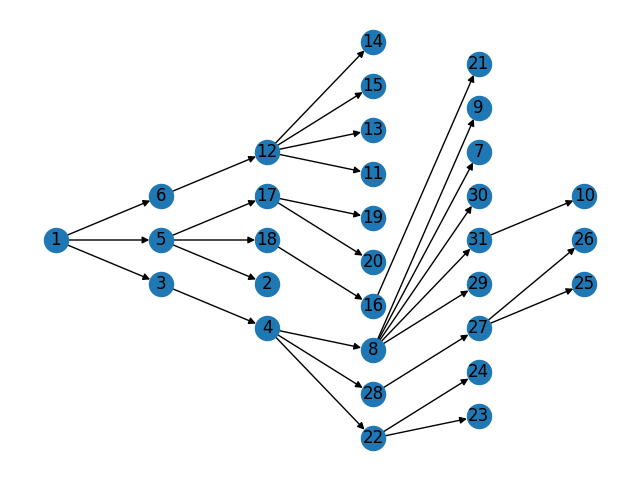
\includegraphics[width=\textwidth]{g4u-bfs.png}
    \caption{Drzewo BFS}
\end{figure}

\begin{figure}[H]
    \centering
    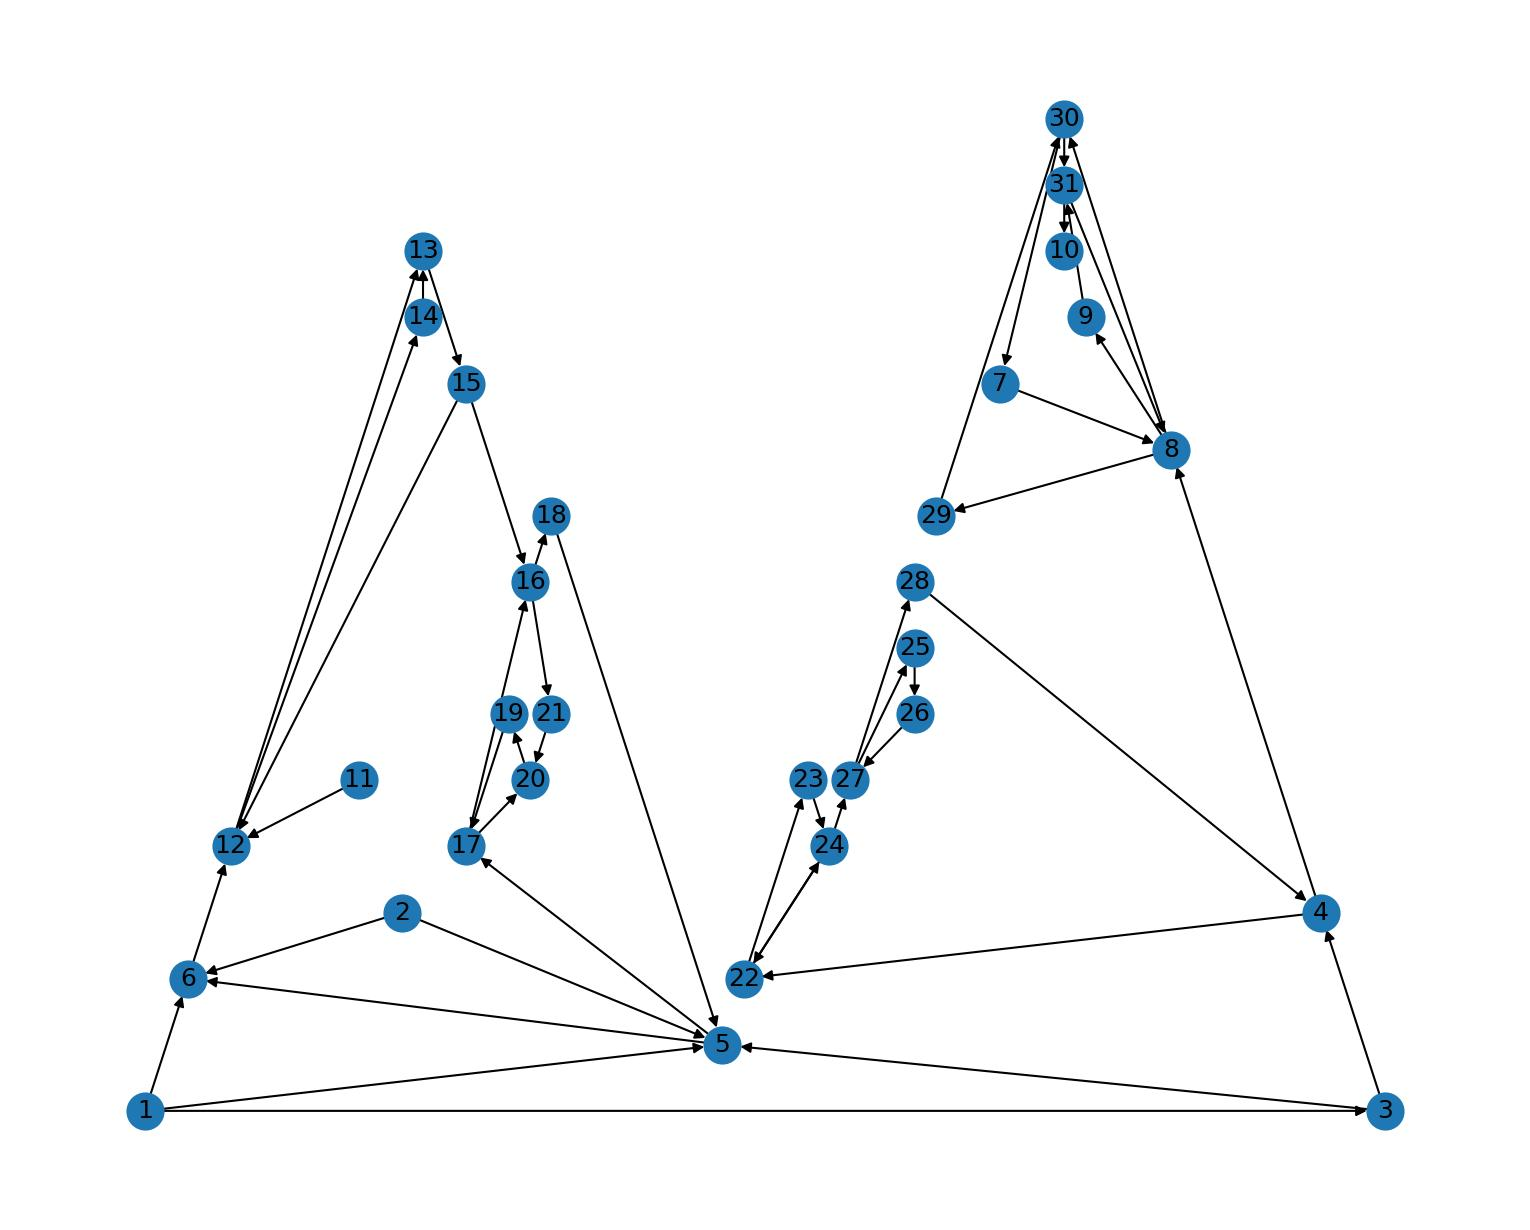
\includegraphics[width=\textwidth]{g4d.jpg}
    \caption{Graf skierowany}
\end{figure}

\begin{figure}[H]
    \centering
    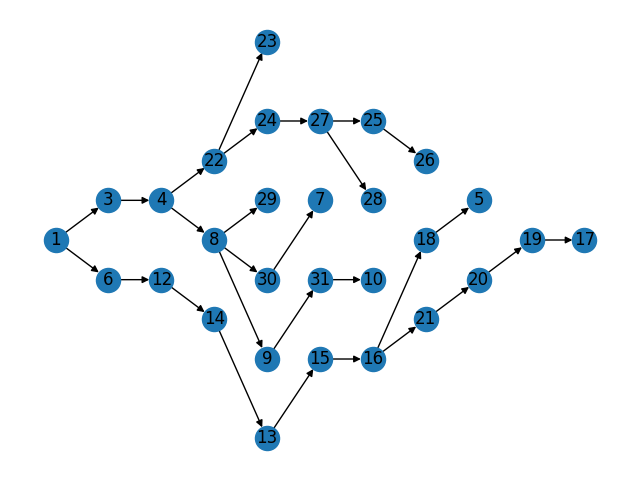
\includegraphics[width=\textwidth]{g4d-dfs.png}
    \caption{Drzewo DFS}
\end{figure}

\begin{figure}[H]
    \centering
    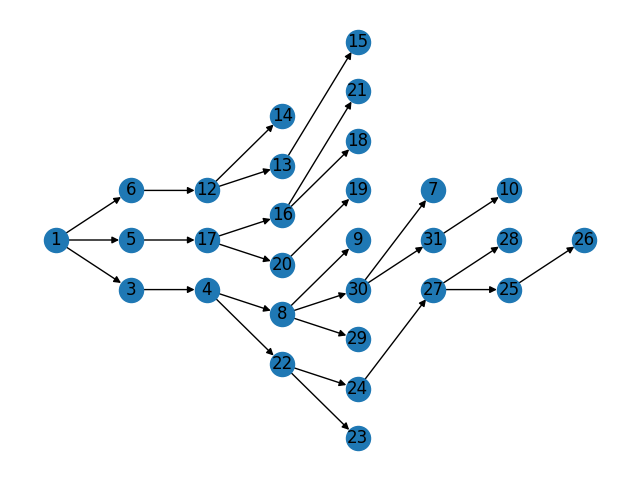
\includegraphics[width=\textwidth]{g4d-bfs.png}
    \caption{Drzewo BFS}
\end{figure}

\subsection{Wyniki}

\begin{table}[H]\centering
    \caption{DFS}
    \begin{tabular}{|p{1cm}|p{10cm}|}\hline
        nr grafu & wynik
        \\\hline
        1        & 1-> 6-> 12-> 14-> 13-> 15-> 16-> 21-> 20-> 19-> 17-> 5->
        18-> 3->
        4-> 8-> 9-> 31-> 10-> 30-> 7-> 29-> 28-> 27-> 26-> 25-> 24-> 22-> 23->
        2-> 11
        \\\hline
        2        & 1-> 6-> 12-> 14-> 13-> 15-> 16-> 21-> 20-> 19-> 17-> 18->
        5-> 3->
        4-> 8-> 9-> 31-> 10-> 30-> 7-> 29-> 22-> 24-> 27-> 28-> 25-> 26-> 23
        \\\hline
    \end{tabular}
\end{table}

\begin{table}[H]\centering
    \caption{BFS}
    \begin{tabular}{|p{1cm}|p{10cm}|}\hline
        nr grafu & wynik
        \\\hline
        1        & 1-> 3-> 5-> 6-> 4-> 2-> 18-> 17-> 12-> 22-> 28-> 8-> 16->
        20-> 19-> 11-> 13-> 15-> 14-> 23-> 24-> 27-> 29-> 31-> 30-> 7-> 9->
        21-> 25->
        26-> 10
        \\\hline
        2        & 1-> 3-> 5-> 6-> 4-> 17-> 12-> 22-> 8-> 20-> 16-> 13-> 14->
        23-> 24-> 29-> 30-> 9-> 19-> 18-> 21-> 15-> 27-> 31-> 7-> 25-> 28->
        10-> 26
        \\\hline
    \end{tabular}
\end{table}

\subsection{Czasy}

\begin{table}[H]\centering
    \caption{DFS}
    \begin{tabular}{|c|c|c|c|c|}\hline
        nazwa    & skierowany & |V| + |E| & czas [$\mu s$] \\\hline
        g3-1.txt & skierowany & 55        & 8759      \\\hline
        g3-2.txt & skierowany & 292       & 12228     \\\hline
        g3-3.txt & skierowany & 2617      & 575506    \\\hline
        g3-4.txt & skierowany & 25952     & 662466    \\\hline
        g3-5.txt & skierowany & 259689    & 1650979   \\\hline
        g3-6.txt & skierowany & 2598908   & 13701511  \\\hline
    \end{tabular}
\end{table}

\begin{table}[H]\centering
    \caption{BFS}
    \begin{tabular}{|c|c|c|c|c|}\hline
        nazwa    & skierowany & |V| + |E| & czas [$\mu s$] \\\hline
        g3-1.txt & skierowany & 55        & 1793      \\\hline
        g3-2.txt & skierowany & 292       & 2286      \\\hline
        g3-3.txt & skierowany & 2617      & 12561     \\\hline
        g3-4.txt & skierowany & 25952     & 115375    \\\hline
        g3-5.txt & skierowany & 259689    & 1579917   \\\hline
        g3-6.txt & skierowany & 2598908   & 17243703  \\\hline
    \end{tabular}
\end{table}

\clearpage

\section{Sortowanie topologiczne}

\subsection{Algorytm}

Zastosowałem wersję algorytmy Kahna.

\begin{itemize}
    \item Dla każdego wierzchołka przechwuję liczbę wchodzących krawędzi $c$.
    \item Wierzchołki o $c=0$ wrzucam na stos.
    \item Przy usuwaniu wierzchołka ze stosu dekremetuję $c$ jego sukcesorów,
          i każdy sukcesor o $c=0$ wrzucam na stos.
    \item Kolejność wierzchołków zrzucanych ze stosu to porządek topologiczny.
    \item Jeżeli po opróżnieniu stosu istnieje wierzchołek o $c \neq 0$,
          to graf posiada skierowany cykl.
\end{itemize}

Algorytm ma złożoność liniową - $O(V + E)$.

\subsection{Grafy}

\begin{figure}[H]
    \centering
    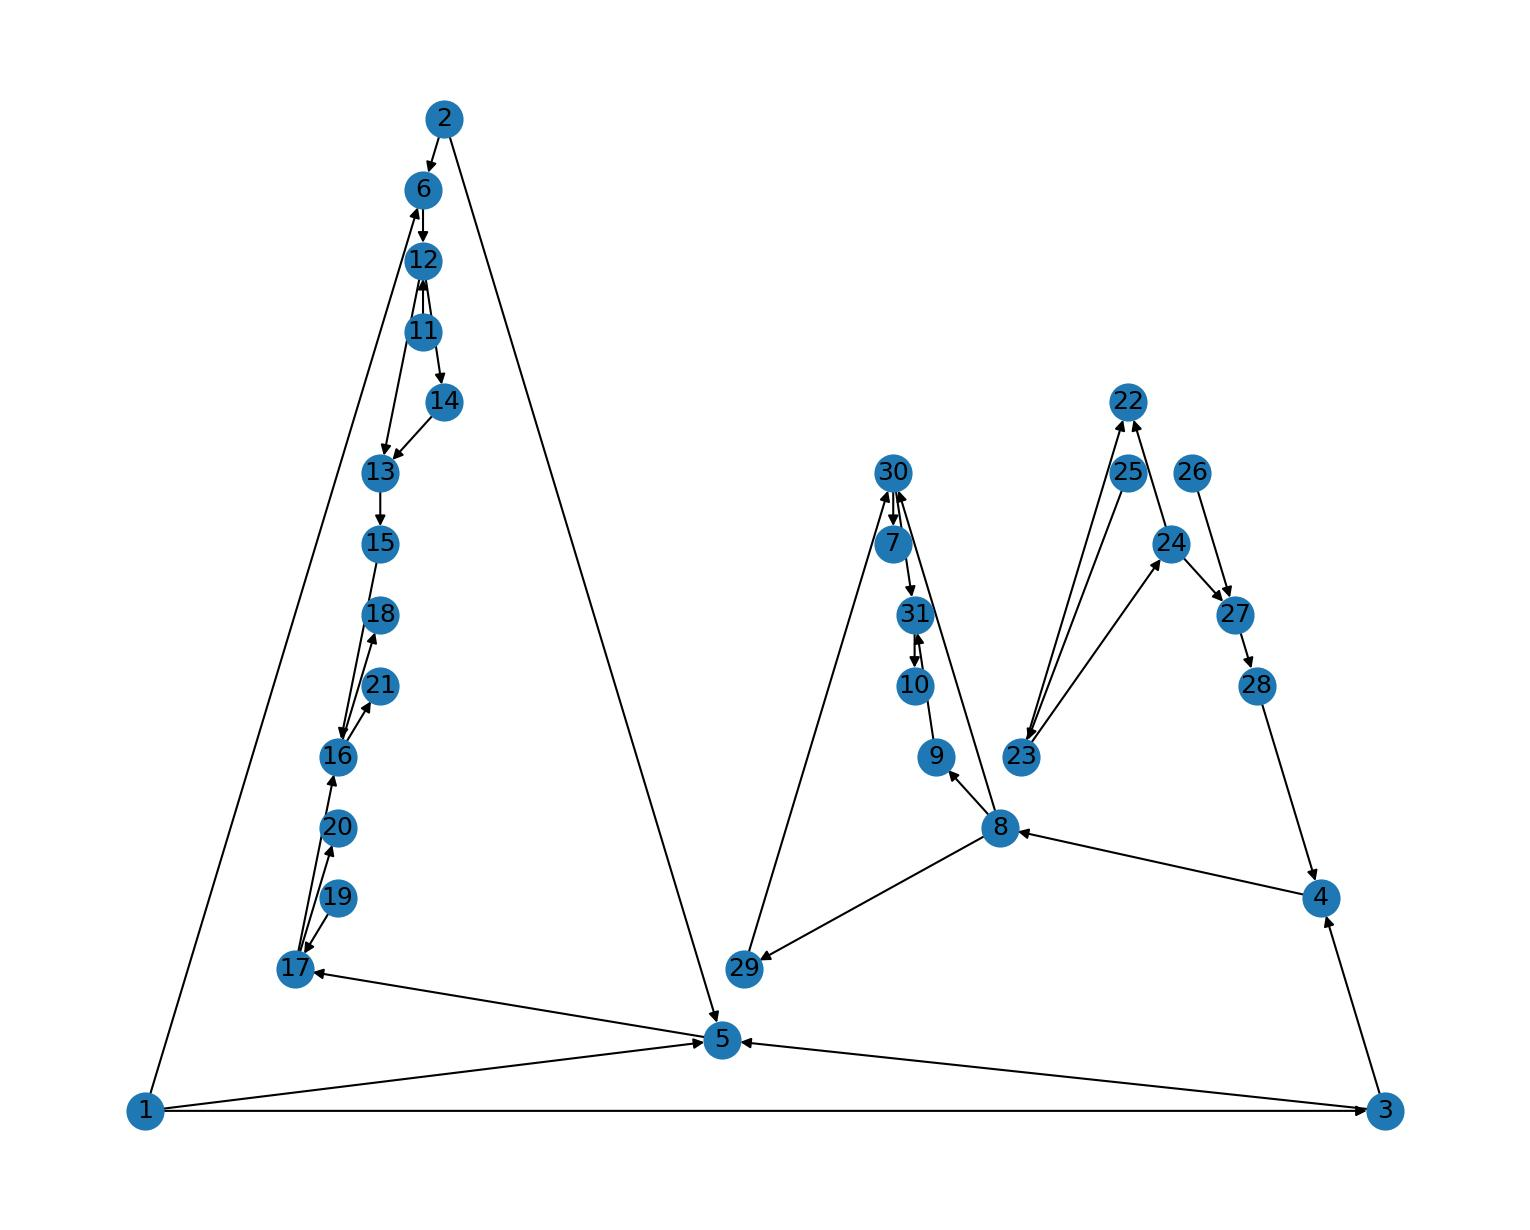
\includegraphics[width=\textwidth]{g2a-moj.jpg}
    \caption{Graf bez cyklu skierowanego}
\end{figure}

\begin{figure}[H]
    \centering
    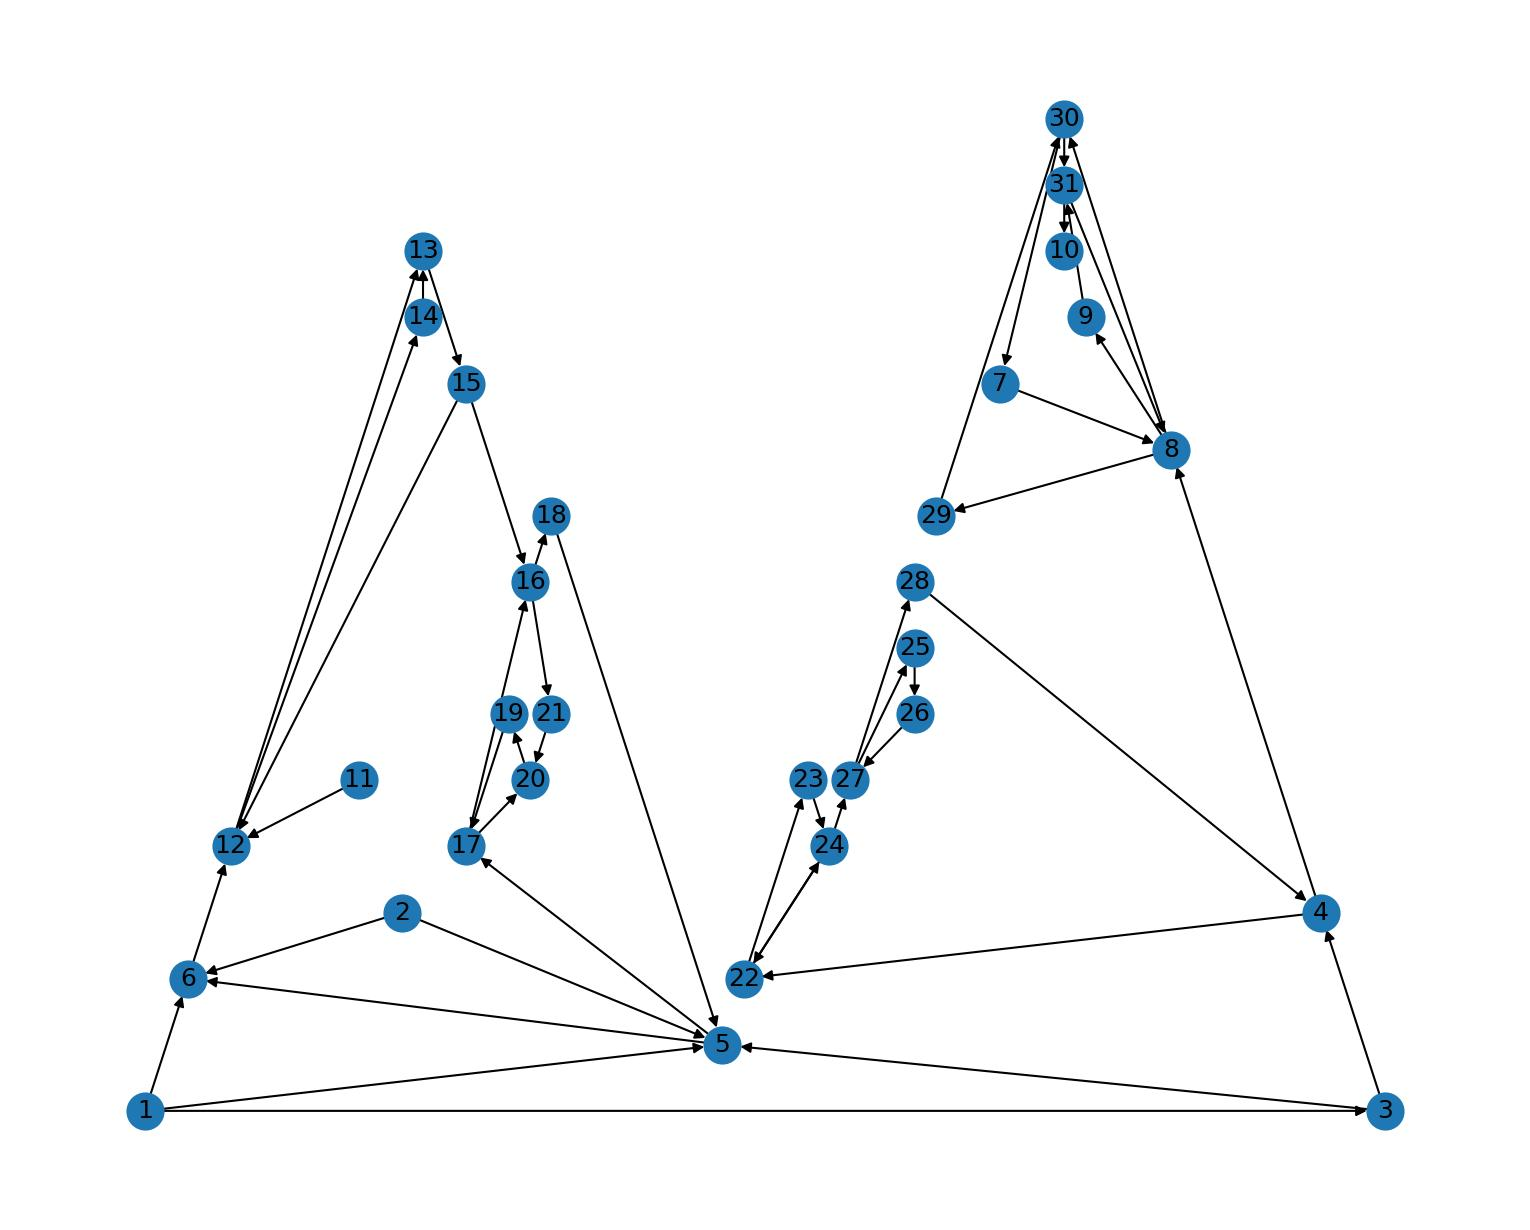
\includegraphics[width=\textwidth]{g2b-moj.jpg}
    \caption{Graf z cyklem skierowanym}
\end{figure}

\subsection{Wyniki}

\begin{table}[H]\centering
    \caption{BFS}
    \begin{tabular}{|p{1cm}|p{10cm}|}\hline
        nr grafu & wynik
        \\\hline
        1        & 26-> 25-> 23-> 24-> 27-> 28-> 22-> 19-> 11-> 2-> 1-> 6-> 12-> 14->
        13-> 15-> 3-> 5-> 17-> 16-> 21-> 18-> 20-> 4-> 8-> 9-> 29-> 30-> 7-> 31-> 10
        \\\hline
        2        & Graf zawiera skierowany cykl
        \\\hline
    \end{tabular}
\end{table}

\subsection{Czasy}

\begin{table}[H]\centering
    \caption{Sortowanie topologiczne}
    \begin{tabular}{|c|c|c|c|c|}\hline
        nazwa     & skierowany & |V| + |E| & czas [$\mu s$] \\\hline
        g2a-1.txt & skierowany & 49        & 2028      \\\hline
        g2b-1.txt & skierowany & 50        & 1636      \\\hline
        g2a-2.txt & skierowany & 361       & 3402      \\\hline
        g2b-2.txt & skierowany & 362       & 2918      \\\hline
        g2a-3.txt & skierowany & 6241      & 3703836   \\\hline
        g2b-3.txt & skierowany & 6242      & 21884     \\\hline
        g2a-4.txt & skierowany & 39601     & 225271    \\\hline
        g2b-4.txt & skierowany & 39602     & 165133    \\\hline
        g2a-5.txt & skierowany & 638401    & 10502435  \\\hline
        g2b-5.txt & skierowany & 638402    & 6528563   \\\hline
        g2a-6.txt & skierowany & 3996001   & 67542464  \\\hline
        g2b-6.txt & skierowany & 3996002   & 44771434  \\\hline
    \end{tabular}
\end{table}

\clearpage

\section{Silnie spójne składowe}

\subsection{Algorytm}

Zastosowałem wersję algorytmu Tarjana do znajdowania silnie spójnych składowych
w grafie skierowanym.
\begin{itemize}
    \item Inicjuję licznik indeksów wierzchołków $index = 0$, a dla każdego
          wierzchołka ustawiam $index[v] = -1$ oraz $lowlink[v] = -1$.
    \item Przechodzę przez każdy wierzchołek grafu, a jeżeli $index[v] = -1$,
          wywołuję procedurę DFS dla wierzchołka $v$.
    \item W procedurze DFS ustawiam $index[v]$ oraz $lowlink[v]$ na bieżący
          indeks, po czym inkrementuję $index$.
    \item Dodaję $v$ na stos i oznaczam go jako będący na stosie.
    \item Dla każdego sąsiada $w$ wierzchołka $v$:
          \begin{itemize}
              \item Jeżeli $w$ nie był odwiedzony, wywołuję rekurencyjnie DFS
                    dla
                    $w$, a następnie aktualizuję $lowlink[v] = \min(lowlink[v],
                        lowlink[w])$.
              \item Jeżeli $w$ jest na stosie, aktualizuję $lowlink[v] =
                        \min(lowlink[v], index[w])$.
          \end{itemize}
    \item Po zakończeniu przetwarzania sąsiadów, jeżeli $lowlink[v] =
              index[v]$, oznacza to początek silnie spójnej składowej:
          \begin{itemize}
              \item Usuwam wierzchołki ze stosu, aż do $v$, tworząc nową
                    składową.
          \end{itemize}
\end{itemize}

Algorytm Tarjana wykonuje tę procedurę dla każdego wierzchołka, odwiedzając
każdy tylko raz, dzięki czemu jego złożoność czasowa wynosi $O(V + E)$, gdzie
$V$ to liczba wierzchołków, a $E$ to liczba krawędzi w grafie.

\subsection{Grafy}

\begin{figure}[H]
    \centering
    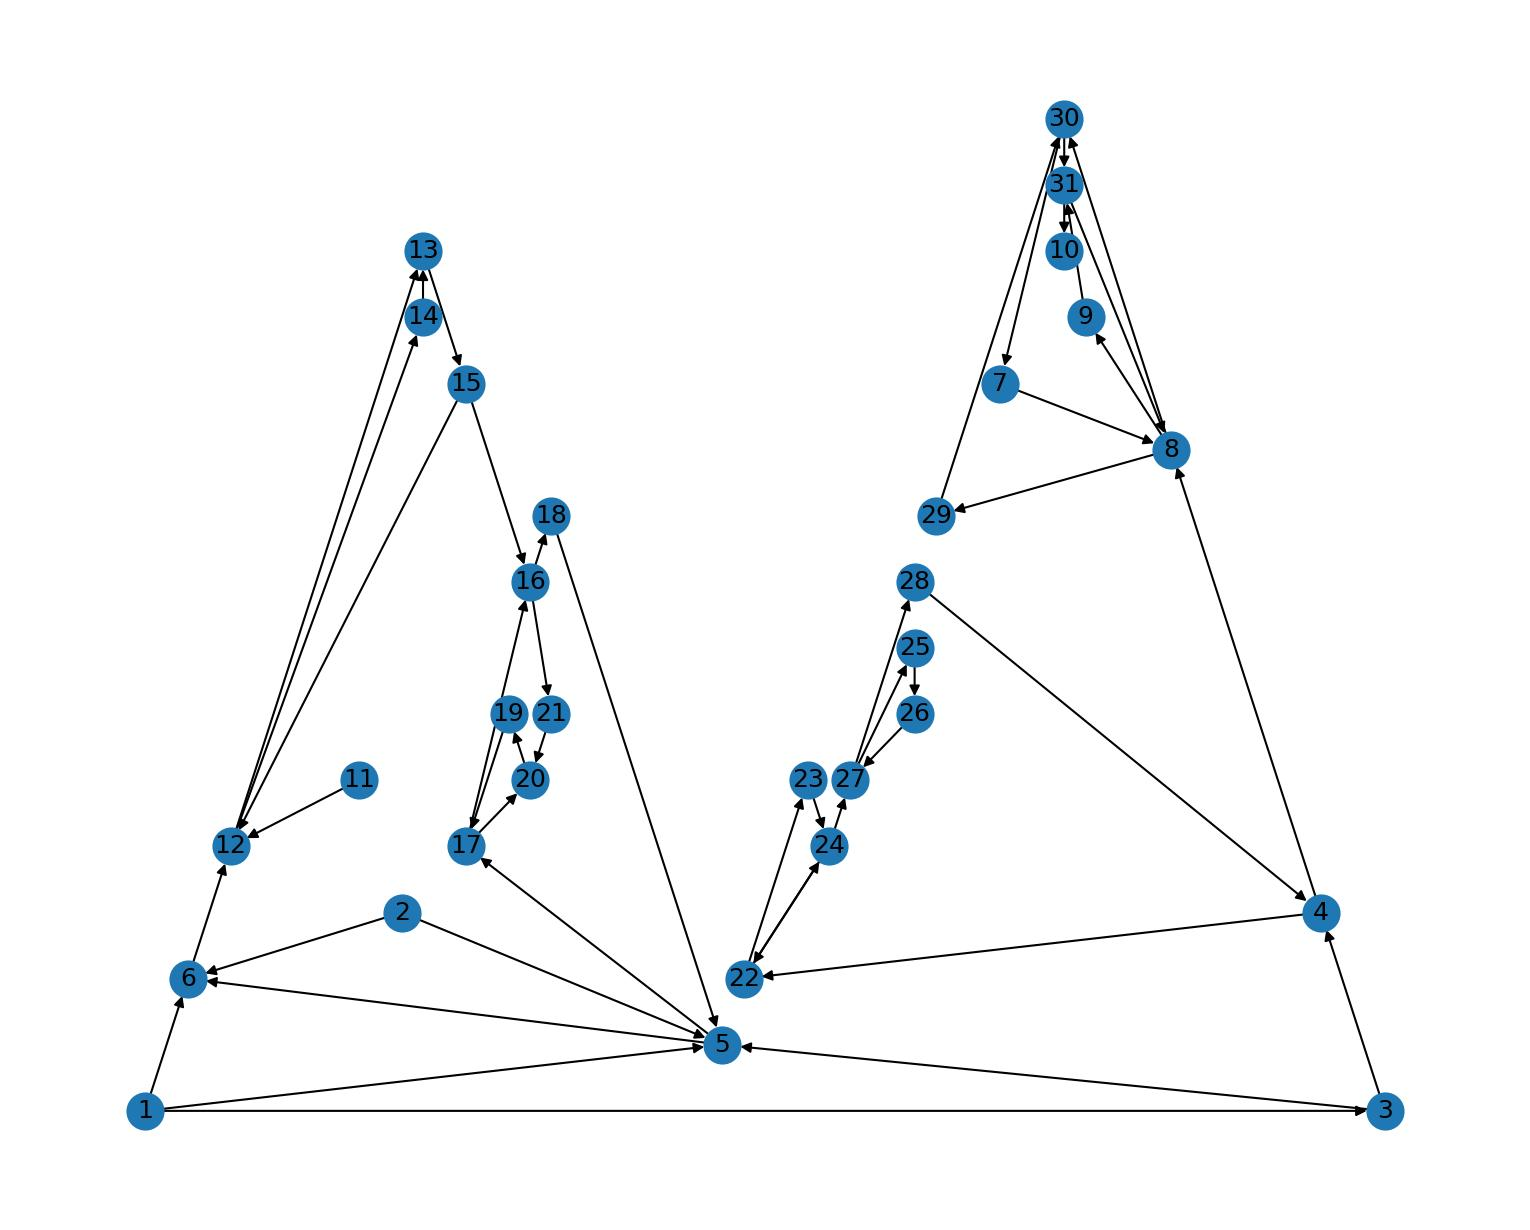
\includegraphics[width=\textwidth]{g3-moj1.jpg}
    \caption{Graf złożony z 8 silnie spójnych składowych}
\end{figure}

\begin{figure}[H]
    \centering
    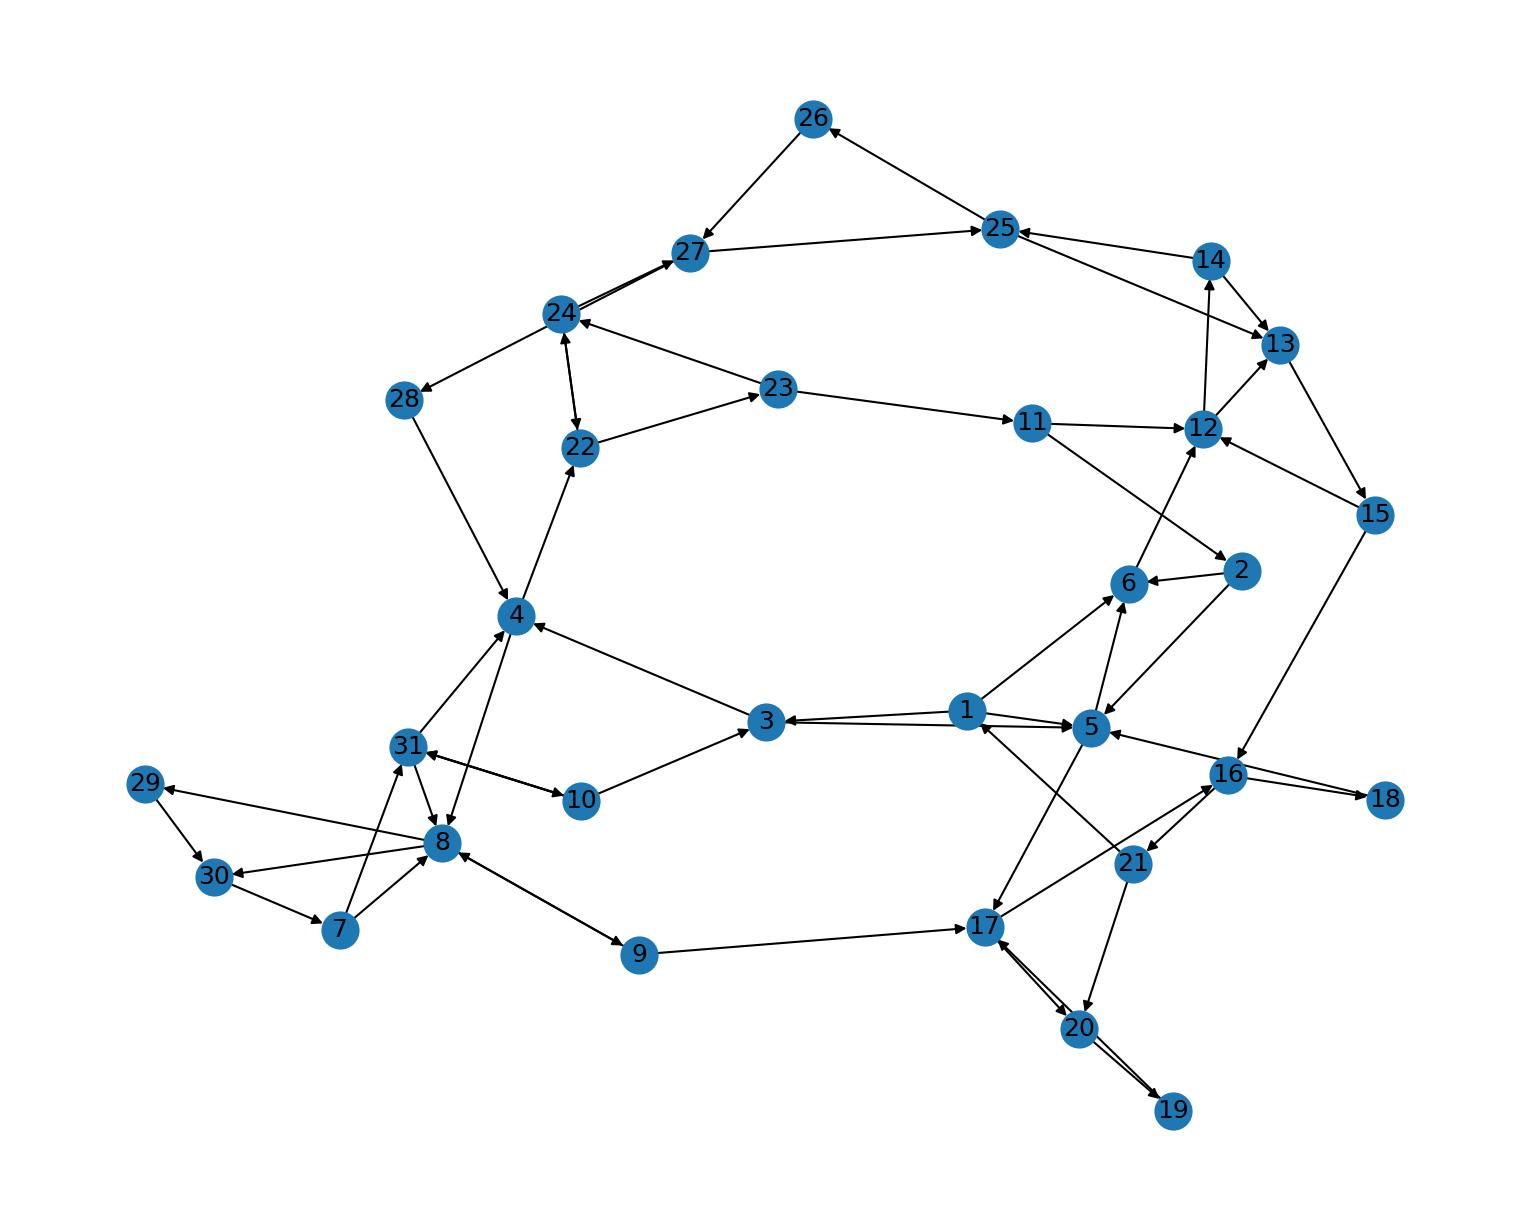
\includegraphics[width=\textwidth]{g3-moj2.jpg}
    \caption{Graf silnie spójny}
\end{figure}

\subsection{Wyniki}

\begin{table}[H]\centering
    \caption{BFS}
    \begin{tabular}{|p{1cm}|p{10cm}|}\hline
        nr grafu & wynik
        \\\hline
        1        & Liczba silnie spójnych składowych 8
        Rozmiar komponentu 1: 1
        10
        Rozmiar komponentu 2: 6
        9, 7, 31, 30, 29, 8
        Rozmiar komponentu 3: 8
        28, 26, 25, 27, 24, 23, 22, 4
        Rozmiar komponentu 4: 12
        14, 17, 19, 20, 21, 18, 16, 15, 13, 12, 6, 5
        Rozmiar komponentu 5: 1
        3
        Rozmiar komponentu 6: 1
        1
        Rozmiar komponentu 7: 1
        2
        Rozmiar komponentu 8: 1
        11
        \\\hline
        2        & Liczba silnie spójnych składowych 1
        Rozmiar komponentu 1: 31
        9, 10, 31, 7, 30, 29, 8, 2, 11, 28, 21, 19, 20, 17, 6, 5, 18, 16, 14,
        12, 15, 13, 26, 25, 27, 24, 23, 22, 4, 3, 1
        \\\hline
    \end{tabular}
\end{table}

\subsection{Czasy}

\begin{table}[H]\centering
    \caption{Silnie spójne składowe}
    \begin{tabular}{|c|c|c|c|c|}\hline
        nazwa    & skierowany & |V| + |E| & czas [$\mu s$] \\\hline
        g3-1.txt & skierowany & 55        & 9250      \\\hline
        g3-2.txt & skierowany & 292       & 23920     \\\hline
        g3-3.txt & skierowany & 2617      & 4544626   \\\hline
        g3-4.txt & skierowany & 25952     & 675758    \\\hline
        g3-5.txt & skierowany & 259689    & 10483782  \\\hline
        g3-6.txt & skierowany & 2598908   & 109814100 \\\hline
    \end{tabular}
\end{table}

\clearpage

\section{Dwudzielność}

\subsection{Algorytm}

Zastosowałem zmodyfikowany algorytm DFS,
który koloruje wierchołki na czarno i biało.
Dla każdego sukcesora odwiedzonego wierzchołka w algorytmie:

\begin{itemize}
    \item Jeśli sukcesor $v$ nie był odwiedzony to koloruję go na kolor
          przeciwny v.
    \item W przeciwnym wypadku, jeśli kolor sukcesora różni się o koloru $v$,
          to graf nie jest dwudzielny.
\end{itemize}

Złożoność algorytmu jest liniowa, jak DFS, bo
zastosowane modyfikacje dodają stałą liczbę operacji.

Dla grafów skierownych, aby algorytm działał poprawnie,
należy traktować je jako nieskierowane.

\subsection{Grafy}

\begin{figure}[H]
    \centering
    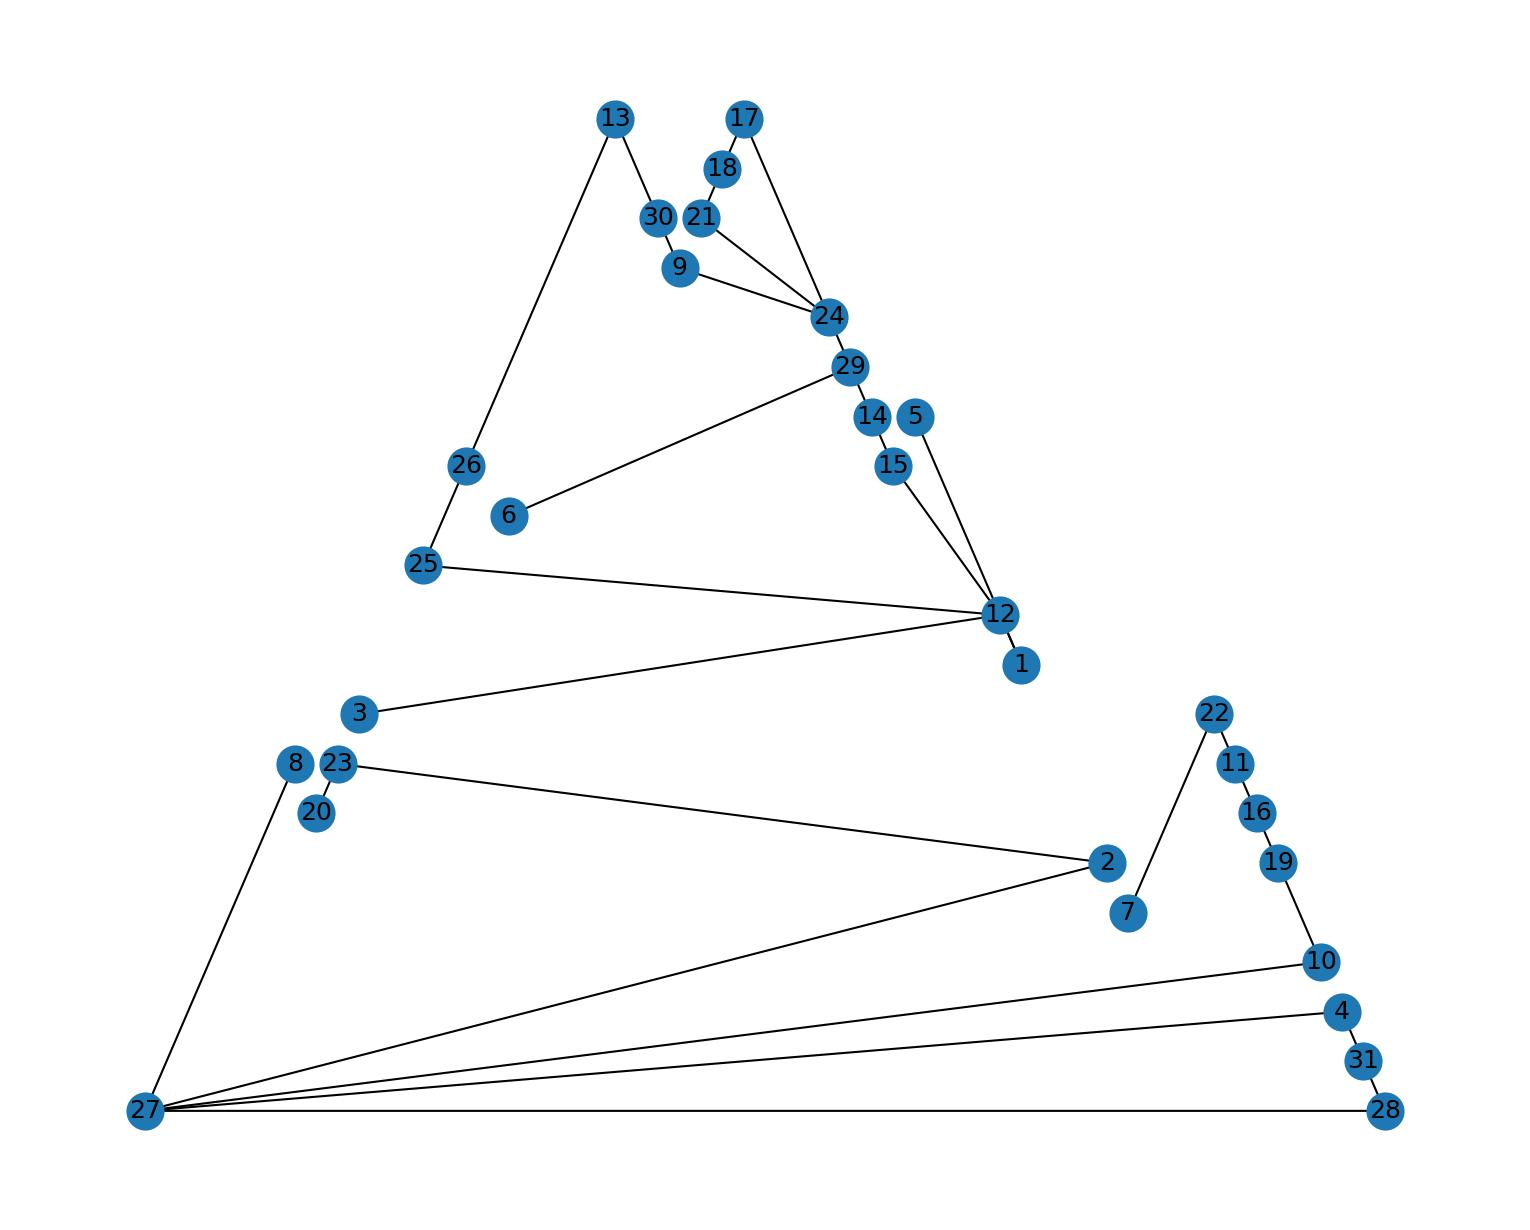
\includegraphics[width=\textwidth]{u4a-moj.jpg}
    \caption{Graf nieskierowany dwudzielny}
\end{figure}

\begin{figure}[H]
    \centering
    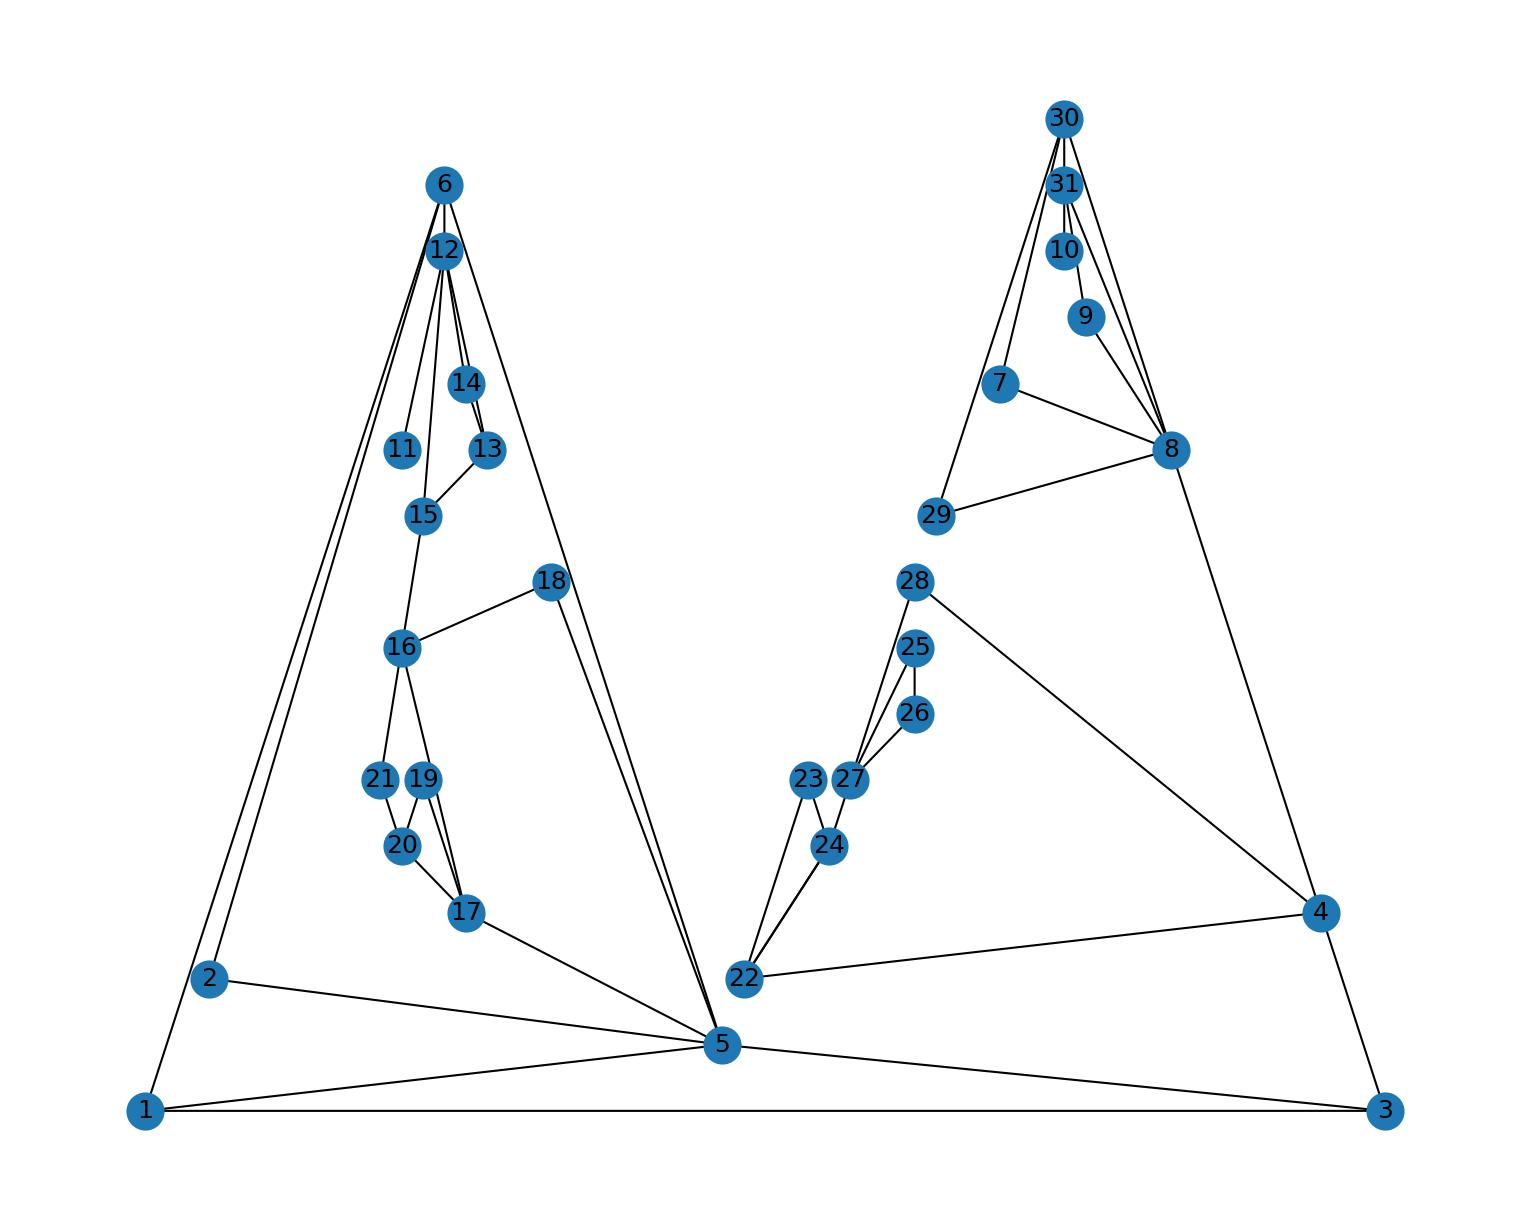
\includegraphics[width=\textwidth]{u4b-moj.jpg}
    \caption{Graf nieskierowany niedwudzielny}
\end{figure}

\begin{figure}[H]
    \centering
    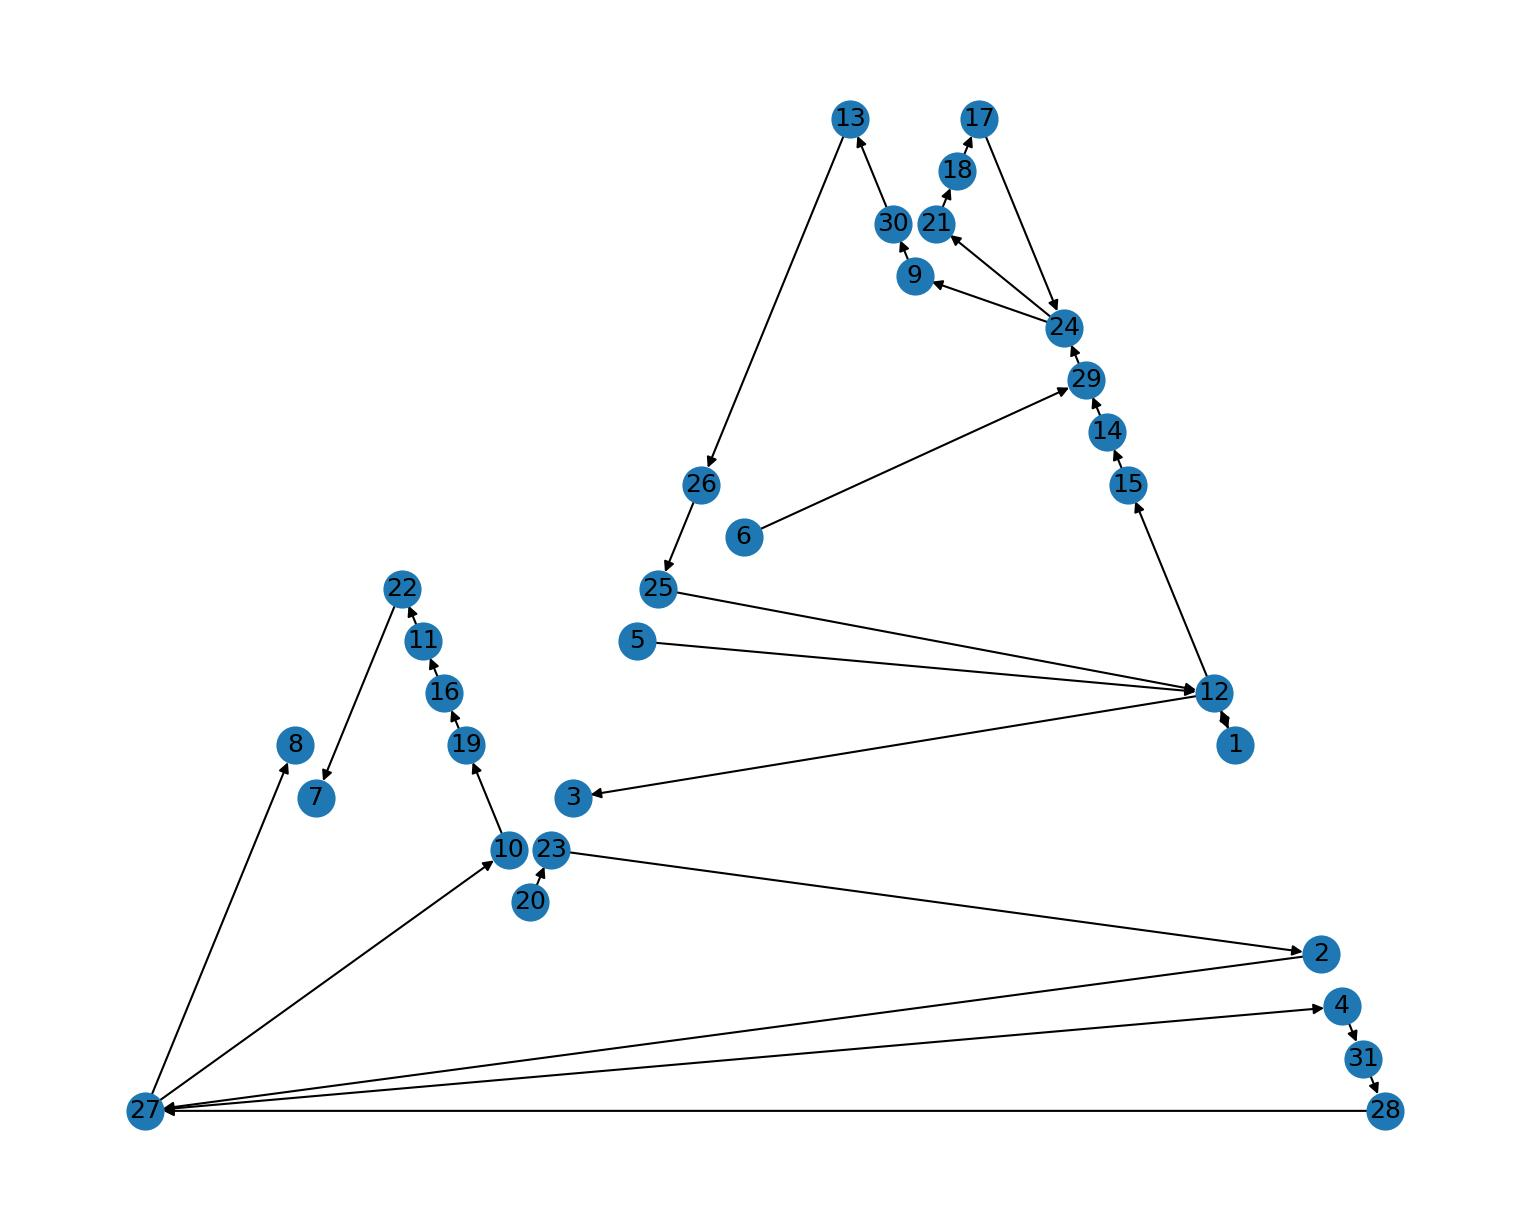
\includegraphics[width=\textwidth]{d4a-moj.jpg}
    \caption{Graf skierowany dwudzielny}
\end{figure}

\begin{figure}[H]
    \centering
    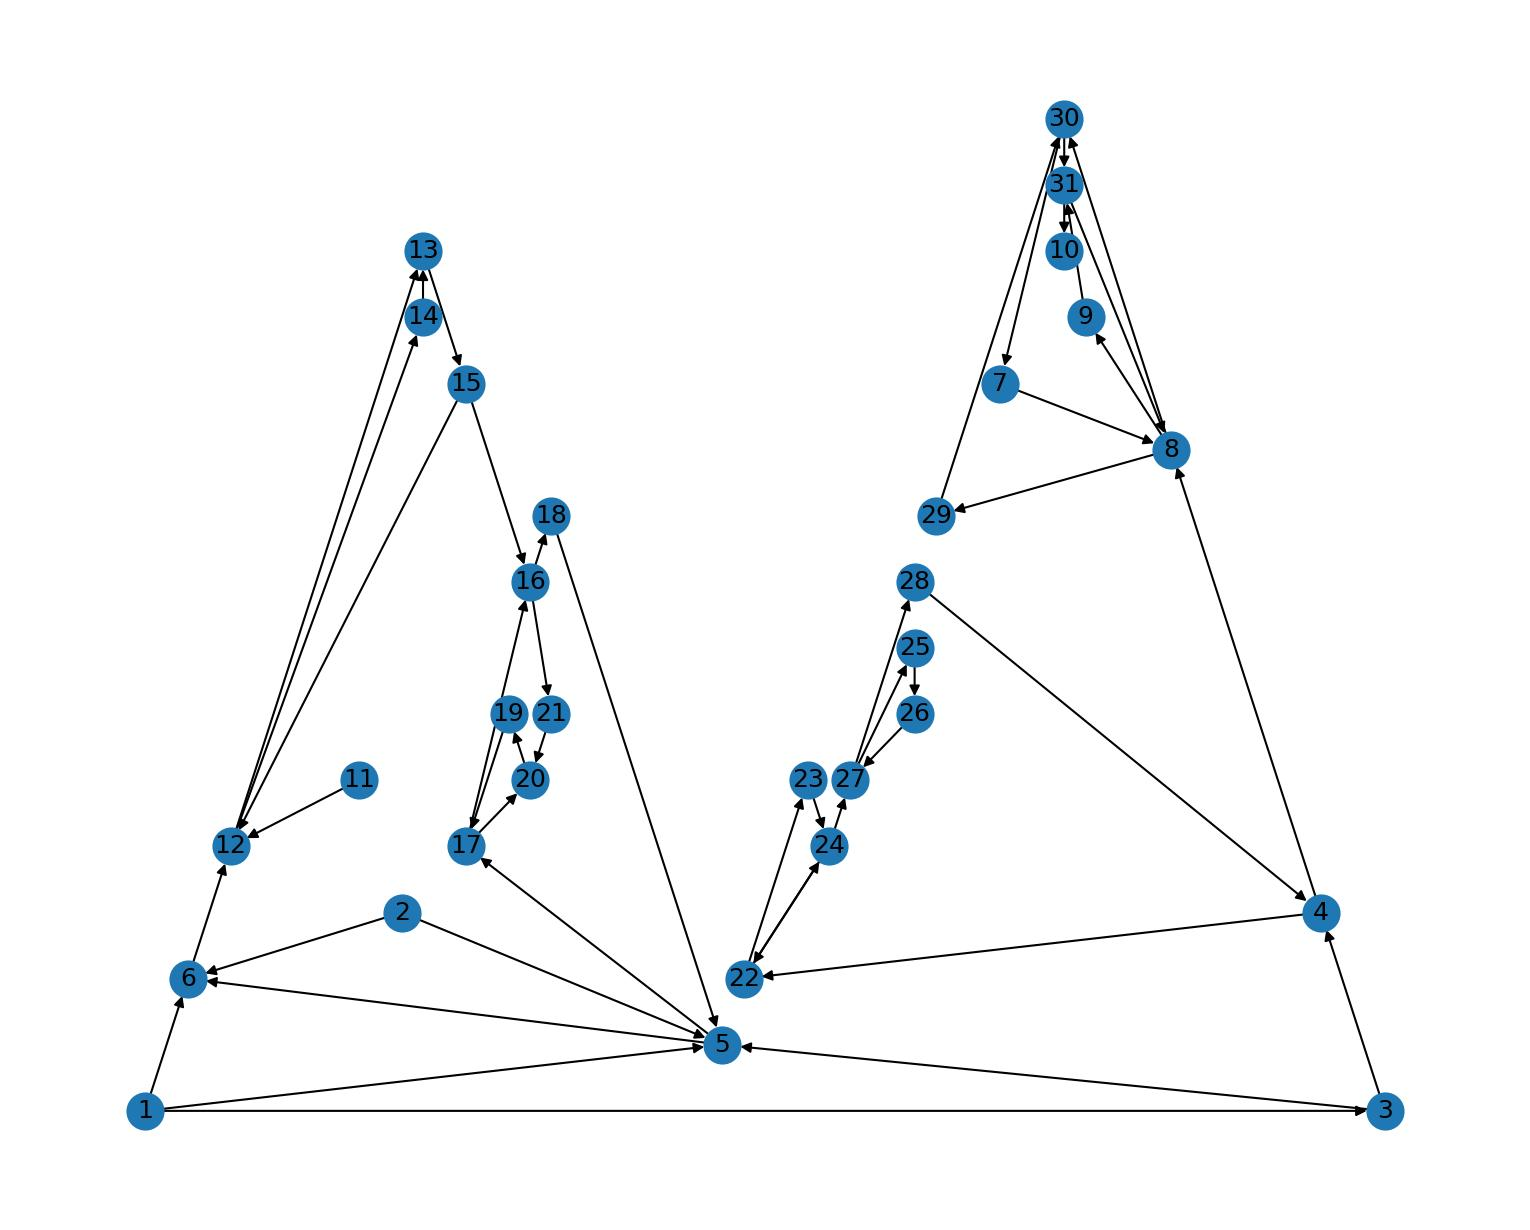
\includegraphics[width=\textwidth]{d4b-moj.jpg}
    \caption{Graf skierowany niedwudzielny}
\end{figure}

\subsection{Wyniki}

\begin{table}[H]\centering
    \caption{BFS}
    \begin{tabular}{|p{1cm}|p{10cm}|}\hline
        nr grafu & wynik
        \\\hline
        1        & Wierzchołki niebieskie:
        6, 7, 11, 12, 14, 18, 19, 23, 24, 26, 27, 30, 31
        Wierzchołki czerwone:
        1, 2, 3, 4, 5, 8, 9, 10, 13, 15, 16, 17, 20, 21, 22, 25, 28, 29
        \\\hline
        2        & Graf nie jest dwudzielny
        \\\hline
        3        & Wierzchołki niebieskie:
        6, 7, 11, 12, 14, 18, 19, 23, 24, 26, 27, 30, 31
        Wierzchołki czerwone:
        1, 2, 3, 4, 5, 8, 9, 10, 13, 15, 16, 17, 20, 21, 22, 25, 28, 29
        \\\hline
        4        & Graf nie jest dwudzielny
        \\\hline
    \end{tabular}
\end{table}

\subsection{Czasy}

\begin{table}[H]\centering
    \caption{Dwudzielność}
    \begin{tabular}{|c|c|c|c|c|}\hline
        nazwa     & skierowany    & |V| + |E| & czas [$\mu s$] \\\hline
        d4a-1.txt & skierowany    & 40        & 7816      \\\hline
        d4b-1.txt & skierowany    & 41        & 5743      \\\hline
        u4a-1.txt & nieskierowany & 37        & 3861      \\\hline
        u4b-1.txt & nieskierowany & 37        & 2871      \\\hline
        d4a-2.txt & skierowany    & 280       & 22518     \\\hline
        d4b-2.txt & skierowany    & 281       & 26752     \\\hline
        u4a-2.txt & nieskierowany & 317       & 17342     \\\hline
        u4b-2.txt & nieskierowany & 317       & 12263     \\\hline
        d4a-3.txt & skierowany    & 4720      & 167435    \\\hline
        d4b-3.txt & skierowany    & 4721      & 137632    \\\hline
        u4a-3.txt & nieskierowany & 2557      & 116079    \\\hline
        u4b-3.txt & nieskierowany & 2557      & 42739     \\\hline
        d4a-4.txt & skierowany    & 29800     & 5713498   \\\hline
        d4b-4.txt & skierowany    & 29801     & 930030    \\\hline
        u4a-4.txt & nieskierowany & 40957     & 1163949   \\\hline
        u4b-4.txt & nieskierowany & 40957     & 738358    \\\hline
        d4a-5.txt & skierowany    & 479200    & 26118637  \\\hline
        d4b-5.txt & skierowany    & 479201    & 20099911  \\\hline
        u4a-5.txt & nieskierowany & 327677    & 9742945   \\\hline
        u4b-5.txt & nieskierowany & 327677    & 6568739   \\\hline
        d4a-6.txt & skierowany    & 2998000   & 170479454 \\\hline
        d4b-6.txt & skierowany    & 2998001   & 111266864 \\\hline
        u4a-6.txt & nieskierowany & 2621437   & 79547959  \\\hline
        u4b-6.txt & nieskierowany & 2621437   & 53376522  \\\hline
    \end{tabular}
\end{table}

\end{document}
